\subsection{Using statistics to calculate uncertainty}

By now in a experimental design, I am usually at my tolerance limit for
calculating uncertainties. You might ask, can't we get our powerful
computers to help us out a little bit with finding the uncertainty? After
all, we went to all the trouble to get the data on the computer. The answer
is, yes!

Let's suppose we have done our experiment and we have some data that look
like this: 

\begin{figure}[h!]
	\centering
	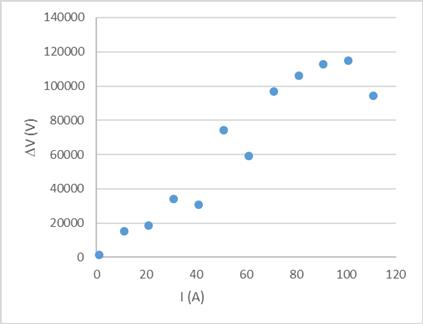
\includegraphics[width=3.563in,height=2.7345in]{PH4CAV2W}
\end{figure}

This looks pretty good. It seems to be sort of linear. We might guess from
this that Ohm's law is begin obeyed. But we want $R_{test}$ and $R_{test}$
is the slope of this line. We could calculate $R_{test}$ from each pair of $%
\Delta V$ and $I$ points and find it's uncertainty using standard error
propagation. But it seems that it would be better to take all the points
into our analysis to find $R_{test}.$ More data should give us a better
estimate for $R_{test}.$ Back in PH150 you may have done such a thing using
a \emph{curve fit}. In the next figure, a curve fit is shown for the data
from the last figure. 

\begin{figure}[h!]
	\centering
	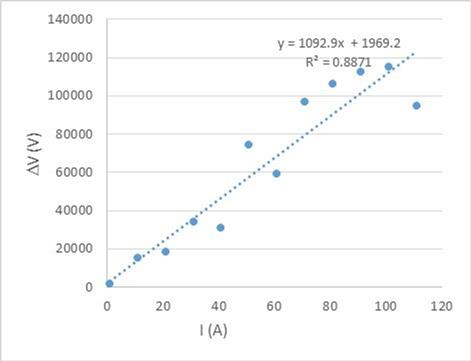
\includegraphics[width=3.966in,height=3.0441in]{PH4CAV2X}
\end{figure}

Notice that I\ performed this curve fit in MicroSoft Excel, but if you are a
great Python programer you could do this directly in Python. You could also
do this in LoggerPro or many other data analysis programs. From the curve
fit equation we can see that we have a slope of $1092.9.$ Since our graph
has $\Delta V$ on the vertical axis and $I$ on the horizontal axis we
recognize 
\begin{eqnarray*}
	\Delta V &=&R_{test}I+0 \\
	y &=&mx+b
\end{eqnarray*}%
that $R_{test}$ must be the slope. In the data above the we can see that the
resistance is a little more than $1092\unit{%
	%TCIMACRO{\U{3a9}}%
	%BeginExpansion
	\Omega%
	%EndExpansion
}$ because that is the slope of our fit line. But we know we need an
uncertainty along with this nominal value. Can we get the computer to do
this as well?

The answer is, of course, Yes! And that will save us a bunch of math! In
some data analysis programs this is easy. LoggerPro, for example, just gives
you the uncertainty in $m$ and $b.$ Excel does not. If you want to use
LoggerPro, that is fine. If you know how to do this in Python, go ahead.
But, if you want to use Excel, let's see how to find the uncertainty.

We will use the \texttt{linst} function in Excel. To find this, select the 
\emph{insert function tool.}

\begin{figure}[h!]
	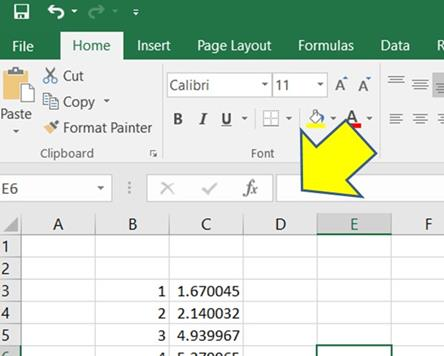
\includegraphics[width=3.7395in,height=3.0018in]{PH4CAV2Y}
\end{figure}This will bring up a dialog box
that allows you to select functions. We want the linst function and it is
categorized under \emph{statistical}, so in the category drop down box 
\begin{figure}[h!]
	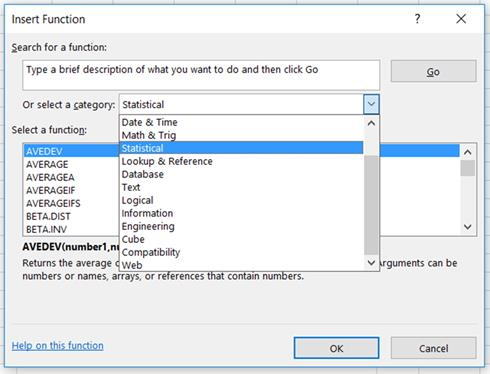
\includegraphics[width=4.1252in,height=3.154in]{PH4CAV2Z}
\end{figure}Then in the \emph{Select a
	function:} box you should find \texttt{LINST} in the list.\begin{figure}[h!]
	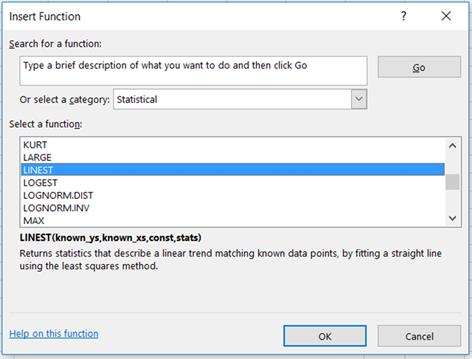
\includegraphics[width=%
	3.9738in,height=3.0277in]{PH4CAV30}
\end{figure}%
When you choose \texttt{LINST}, another dialog box will open.\begin{figure}[h!]
	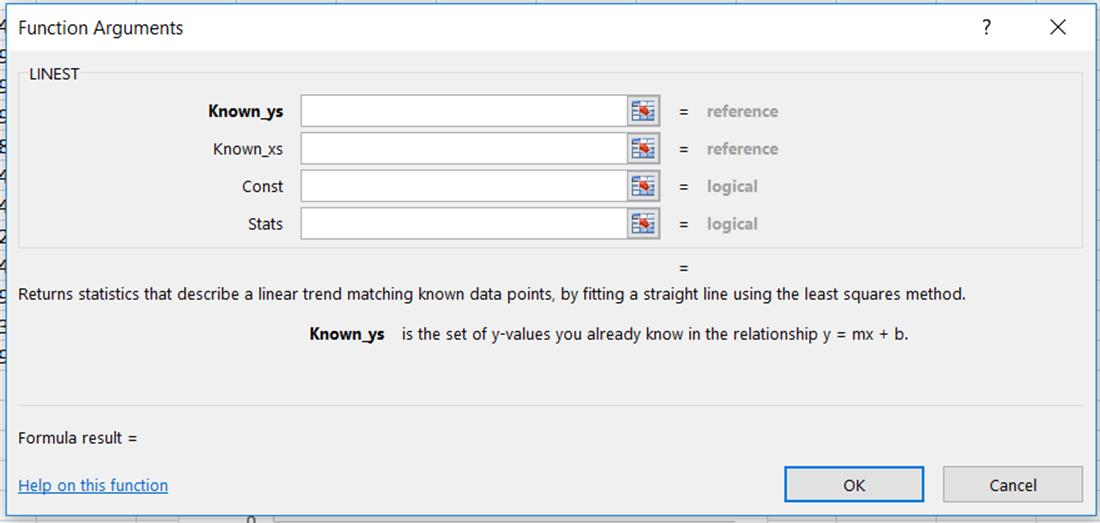
\includegraphics[width=%
	4.7288in,height=2.2554in]{PH4CAV31}
\end{figure}
It will ask you for your $y$-values and your $x$-values. It asks for a
Constant, but leave that input blank. It also asks if we want statistics. We
do, so fill this in with the word \textquotedblleft TRUE\textquotedblright\
in all caps.

When you click on OK, you will get a number in a spreadsheet cell. That is
good, It should be our slope. But we want the uncertainty in that slope. To
do this highlight the cells near the slope value. The region needs to be two
columns by five rows. \begin{figure}[h!]
	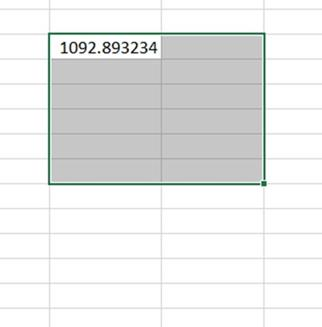
\includegraphics[width=2.7172in,height=2.7596in]{PH4CAV32}
\end{figure}With the region highlighted,
click the formula in the formula bar with your mouse.\begin{figure}[h!]
	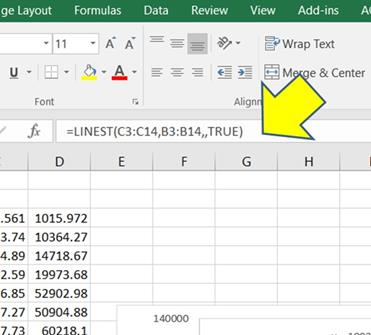
\includegraphics[width=3.128in,height=%
	2.8262in]{PH4CAV33}
\end{figure} It should light up parts of your
spreadsheet. \begin{figure}[h!]
	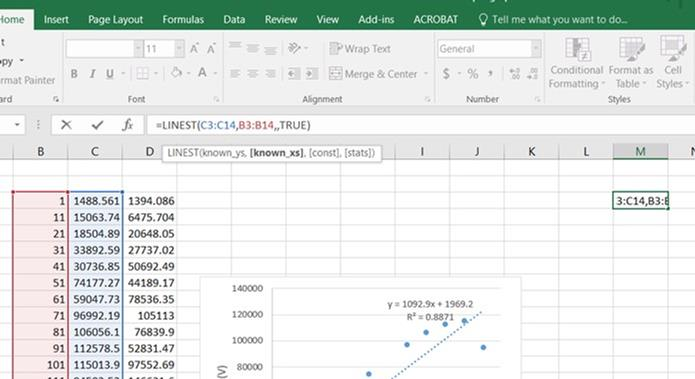
\includegraphics[width=4.2445in,height=2.3212in]{PH4CAV34}
\end{figure}Type CTRL+SHIFT+ENTER all at the
same time. This will fill in the region with statistics on our data. The top
left cell in our region is still the slope, but now right under this slope
is the uncertainty in the slope. We also have in the top, right cell the $y$%
-intercept and below it the $y$-intercept uncertainty. \begin{figure}[h!]
	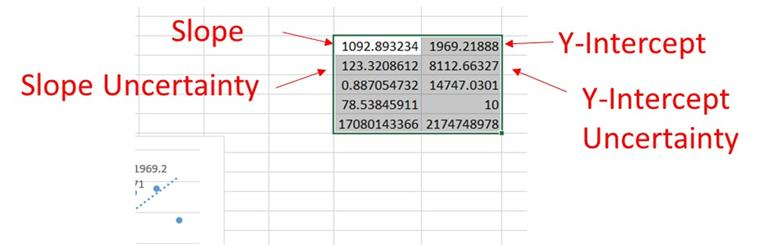
\includegraphics[width=6.3797in%
	,height=2.0721in]{PH4CAW35}
\end{figure}

There are other numbers that are useful, but for now the two rows have given
us what we needed. We have the slope, $m,$ the $y$-intercept, $b,$ and their
uncertainties. For the data in the figures, we would have 
\begin{equation*}
	R_{test}=1100\unit{%
		%TCIMACRO{\U{3a9}}%
		%BeginExpansion
		\Omega%
		%EndExpansion
	}\pm 100\unit{%
		%TCIMACRO{\U{3a9}}%
		%BeginExpansion
		\Omega%
		%EndExpansion
	}
\end{equation*}

This was a little tricky, but was far less mathematical work than doing the
uncertainty for every $\left( I,\Delta V\right) $ pair. We will often use
this technique to find uncertainty.

Also notice that in this analysis technique, we can afford some error in our 
$\Delta V$ and $I$ values. So maybe a $9\%$ error (like we found in one of
our instrument desigs) is not so bad. We may not have to work too hard to
get a wonderful choice of shunt resistor if we are going to use many data
points and the power of statistics to analyze the data in the end!
